%=============================================================================
%
%	Optimization in Banach Spaces
%
%	Continuos evaluation work - Block 3
%
%=============================================================================



%=============================================================================
%	Packages
%=============================================================================

\documentclass[11pt, a4paper]{article}		% document format
\usepackage{graphicx}						% package to insert graphics
\usepackage[english]{babel}
\usepackage[utf8]{inputenc}					% this enables all unicode characters
\usepackage{amsmath, amsfonts, amssymb} 	% maths packages
\usepackage{amsthm}							% theorem styles
\usepackage{fancyhdr}						% package for headers, foot and margin notes
\usepackage{enumitem}						% allows to change the enumeration format in line
\usepackage{tikz}
\usepackage[
  top=2cm,
  bottom=2cm,
  left=3cm,
  right=2cm,
  headheight=17pt, % as per the warning by fancyhdr
  includehead,includefoot,
  heightrounded, % to avoid spurious underfull messages
]{geometry} 




%=============================================================================
%	Commands
%=============================================================================

\providecommand{\U}[1]{\protect\rule{.1in}{.1in}}
\newcommand{\N}{\mathbb{N}}
\newcommand{\E}{\mathcal{E}}
\newcommand{\R}{\mathbb{R}}



%=============================================================================
%	Environment
%=============================================================================

\theoremstyle{plain}
\newtheorem{theorem}{Theorem}%[section]
\newtheorem{lema}[theorem]{Lema}
\newtheorem{definition}[theorem]{Definition}
\newtheorem{exercise}{Exercise}
\newtheorem{algorithm*}{Algorithm}

\theoremstyle{definition}
\newtheorem{solution}{Solution}[exercise]
\renewcommand*{\thesolution}{\theexercise.\alph{solution}}	% Make solution instances enumerate with number of exercise and letter of solution

\usetikzlibrary{calc}



%============================================================================
%	Pagestyle
%=============================================================================

\pagestyle{fancy}		% As we use the fancyhdr pkg need the fancy pagestyle, for more information:
						% http://tug.ctan.org/tex-archive/macros/latex/contrib/fancyhdr/fancyhdr.pdf


%\topmargin 0 pt
%\oddsidemargin 0 pt
%\evensidemargin 0 pt
%\marginparwidth 0 pt


%\textheight 25cm
%\textwidth 400 pt
%\advance\textheight by \topskip

%\parindent 0pt
%\parskip 5mm plus 1mm minus 1mm

\fancyhead[C]{PEC 3}					                	% Central header
\fancyhead[L]{Optimization in Banach Spaces}   				% Left header
\fancyhead[R]{Marc Jovani Bertran}						    % Right header



%=============================================================================
%	Document
%=============================================================================

\begin{document}
	\section*{1}

\begin{definition}
    Sea $(X, \| \cdot \|)$ un espacio vectorial normado y $D \subset X$ un cono convexo,
    con $X \neq D \neq \{ 0_X \}$.
    \begin{enumerate}[label=\textup{(\alph*)}]
        \item Base de un cono.
            \textup{
                Se dice que un conjunto no vacío y convexo $B \subset D$ es una base de $D$,
                si cada elemento $x \in D \setminus \{ 0_X \}$ admite una única representación de la forma
                \begin{equation*}
                    x = \lambda b, \text{ con } \lambda > 0 \text{ y } b \in B.
                \end{equation*}
            }

        \item Cono polar.
            \textup{
                El cono
                \begin{equation*}
                    D^* := \{ \mu \in X^* : \mu(d) \geq 0, \; \forall d \in D \},
                \end{equation*}
                recibe el nombre de cono polar o cono dual de $D$
                ($X^*$ denota el espacio dual topológico de $X$).
            }
        \item Cono polar estricto.
            \textup{
                El conjunto 
                \begin{equation*}
                    D^{s*} := \{ \mu \in X^* : \mu(d) > 0, \; \forall d \in D \setminus \{ 0_X \} \},
                \end{equation*}
                recibe el nombre de cono polar estricto de $D$.
            }
    \end{enumerate}
\end{definition}

Para los conceptos introducidos en la definición anterior,
se pide probar las propiedades que se indican a continuación.
En lo que sigue $(X, \| \cdot \|)$ es un espacio vectorial normado y $D \subset X$ un cono convexo, con $X \neq D \neq \{ 0_X \}$.

\noindent \textit{Propiedades.}
\begin{enumerate}
    \item Supóngase que int $D \neq \emptyset$. Se tiene que
        \begin{equation*}
            \text{int} D \subset \{ x \in X : \mu(x) > 0, \forall \mu \in D^{*} \setminus \{ 0_{X^*} \} \}.
        \end{equation*}

    \item Si int $D \neq \emptyset$, entonces $D^{*}$ es puntiagudo (pointed).
    \item Si $D$ tiene una base, entonces $D$ es puntiagudo (pointed).
    \item Supóngase que $D^{s*} \neq \emptyset$.
        Entonces, para cada $\mu \in D^{s*}$ se tiene que el conjunto
        \begin{equation*}
            B := \{ d \in D : \mu(d) = 1 \},
        \end{equation*}
        es una base de $D$.
    \item Si $D^{s*} \neq \emptyset$, entonces $D$ es puntiagudo.
\end{enumerate}

\noindent\rule{10cm}{0.4pt}

\subsection*{1}

Para todo $x \in \text{int}D$ es obvio que $x \in X$,
ademas para todo $\mu \in D^* \setminus \{ 0_{X^*} \}$, tenemos que $\mu(x) \geq 0$.

Sea $x \in \text{int}D$ supongamos que existe $\mu \in D^* \setminus \{ 0_{X^*} \}$ tal que $\mu(x) = 0$.
Entonces como $x \in \text{int}D \neq \emptyset$ tenemos que existe $r > 0$ tal que la bola abierta $B(x, r) \subset \text{int} D$.

Tenemos que existe $w \in \text{int}D \cap B(0, r)$ tal que $w > 0$,
si no existiera tendiéramos que para todo $v \in \text{int}D \cap B(0, r) \subset D$, $\mu(v) = 0$,
por tanto $\mu = 0_{X^*}$, contradiciendo la hipótesis.
Por la linealidad de $\mu$ tenemos que $y = x - w \in B(x, r) \subset \text{int} D \subset D$ y
\begin{equation*}
    \mu(y) = \mu(x) - \mu(w) = - \mu(w) < 0,
\end{equation*} 
contradiciendo que $\mu \in D^*$!!

Por tanto para todo $\mu \in D^* \setminus \{ 0_{X^*} \}$ se tiene que $\mu(x) > 0$,
y esto implica que 
\begin{equation*}
    \text{int} D \subset \{ x \in X : \mu(x) > 0, \forall \mu \in D^{*} \setminus \{ 0_{X^*} \} \}.
\end{equation*}

Notemos que en este caso $D \neq X$ ya que si $D = X$ el único elemento del dual $D^*$ seria $0_{X^*}$,
dado que para cualquier otro funcional $\mu$ si existe $d \in D$ tal que $\mu(d) > 0$,
como $D = X$ tenemos que $-d \in D$ y por tanto $\mu(-d) = - \mu(d) < 0$ contradiciendo que es del dual.

\subsection*{2}

Por el aparatado anterior,
como $\text{int} D \neq \emptyset$ para todo $x \in \text{int}D$ y $\mu \in D^* \setminus \{ 0_{X^*} \}$ tenemos $\mu(x) > 0$.

Si $-\mu \in D^*$ tenemos que para todo $x \in \text{int}D$, $-\mu(x) > 0$,
que implica $\mu(x) < 0$, contradiciendo que $\mu(x) > 0$!!

Resultando en que si $\mu \in D^*$ y $-\mu \in D^*$ entonces $\mu = 0_{X^*}$,
y por tanto $D^*$ es puntiagudo.

\subsection*{3}

Sea $x \in D \setminus \{ 0_X \}$ y $B$ una base de $D$.
Entonces existe un único $b \in B$ y $\lambda > 0$ tal que $x = \lambda b$.

Si $-x \in D \setminus \{ 0_X \}$,
entonces, como $B$ es convexo,
para todo $\alpha \in [0, 1]$ tenemos que
\begin{equation*}
    b_\alpha = \alpha b - (1 - \alpha) b = (2 \alpha - 1) b \in B.
\end{equation*}
Y $x = \lambda b = 2 \lambda b_{0.75}$,
contradiciendo que la representación de $x = \lambda b$ con $\lambda > 0$ y $b \in B$ es única.
Por tanto $x = 0_X$ y consecuentemente $D$ es puntiagudo.

\subsection*{4}

Dado $\mu \in D^{s*}$,
veamos que para cada $x \in D \setminus \{ 0_X \}$ existe un único $b \in B$ y $\lambda > 0$.

Supongamos que existen $b_1, b_2 \in B$ y $\lambda_1, \lambda_2 > 0$,
tales que $x = \lambda_1 b_1 = \lambda_2 b_2$.
Tenemos que
\begin{equation*}
    \mu(x) = \lambda_1 = \lambda_1 \mu(b_1) = \lambda_2 \mu(b_2) = \lambda_2,
\end{equation*}
por tanto $\lambda_1 = \lambda_2$, y como consecuencia
\begin{equation*}
    x = \lambda_1 b_1 = \lambda_1 b_2,
\end{equation*}
Resultando en $b_1 = b_2$.

Veamos ahora que dado $\mu \in D^{s*}$, $B$ genera,
i.e. para todo $x \in D \setminus \{ 0_X \}$ existe $b \in B$ y $\lambda > 0$ tal que $x = \lambda b$.

Supongamos que existe $x \in D \setminus \{ 0_X \}$ tal que para todo $b \in B$ y para todo $\lambda > 0$,
$x \neq \lambda b$.

Como $D$ es un cono se tiene que para todo $\alpha > 0$, $\alpha x \in D$.
% Si $\alpha x = \lambda b$, por algún $b \in B$ y $\lambda > 0$,
% entonces
% \begin{equation*}
%     x = \frac{\lambda}{\alpha} b,
% \end{equation*}
% contradiciendo la hipótesis que no existe $b \in B$ y $\lambda > 0$ tal que $x = \lambda b$.
% Por tanto $\alpha x \neq \lambda b$ para todo $b \in B$ y $\lambda > 0$.
Entonces
\begin{equation*}
    \mu(\alpha x) = \alpha \mu(x),
\end{equation*}
usando $\alpha = \frac{1}{\mu(x)}$,
tenemos que $\mu(\alpha x) = 1$ y por tanto $\alpha x \in B$,
contradiciendo la hipótesis inicial.

\subsection*{5}

Usando el resultado anterior, como $D^{s*} \neq \emptyset$,
tenemos que $D$ tiene una base,
por tanto usando la propiedad 3 tenemos que $D$ es puntiagudo.

	\section*{2}

Obtenga el cono contingente al conjunto
\begin{equation*}
    S := \{ (x, y) \in \R^2 : y \geq (x - 3)^2 + 3 \text{ and } y \leq -x + 8 \},
\end{equation*}
en el punto $(4, 4)$, y determine una base para este cono.

\noindent\rule{10cm}{0.4pt}

Sean $f(x):= (x - 3)^2 + 3$ y $g(x) := -x + 8$, 
derivando tenemos que
\begin{equation*}
    f'(x) = 2(x - 3), \qquad g'(x) = -1,
\end{equation*}
en particular $f'(4) = 2$ y $g'(4) = -1$.
por tanto el cono contingente a $S$ en el punto $(4, 4)$ viene dado por
\begin{equation*}
    T(S, (4, 4)) = \{ \lambda (-1, a) : \lambda \geq 0 \text{ and } a \in [-2, 1] \}.
\end{equation*}

\begin{figure}[h]
\centering
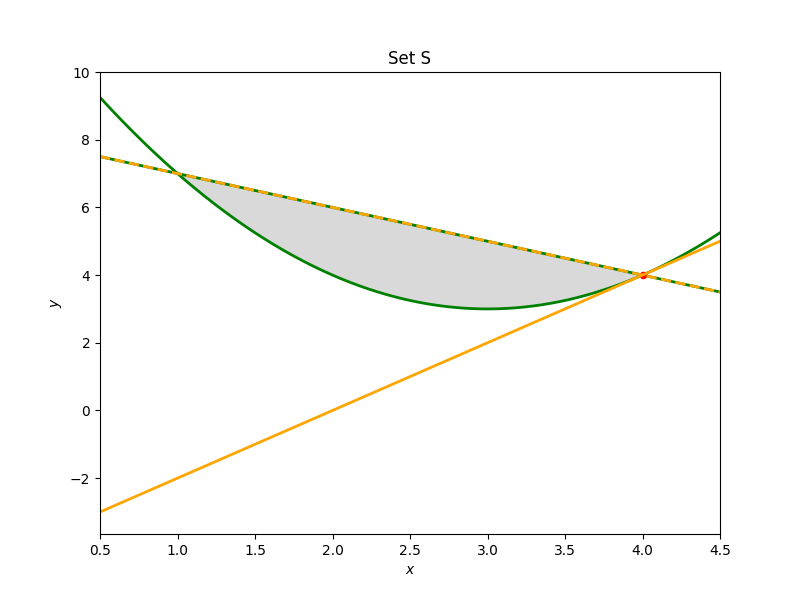
\includegraphics[scale=0.6]{pec3_ex2_setS.png}
\caption{
    Conjunto $S$ y los vectores tangentes en $(4,4)$.
}
\label{ex2_plot_set}
\end{figure}

Una base de $T(S, (4, 4))$ se puede obtener interescando la recta $(-1, y)$ para todo $y$ con el conjunto $T(S, (4,4))$,
de modo que
\begin{equation*}
    B = \{ (-1, y) : y \in [-2, 1] \},
\end{equation*}
es una base de $T(S, (4, 4))$.

\begin{figure}[h]
\centering
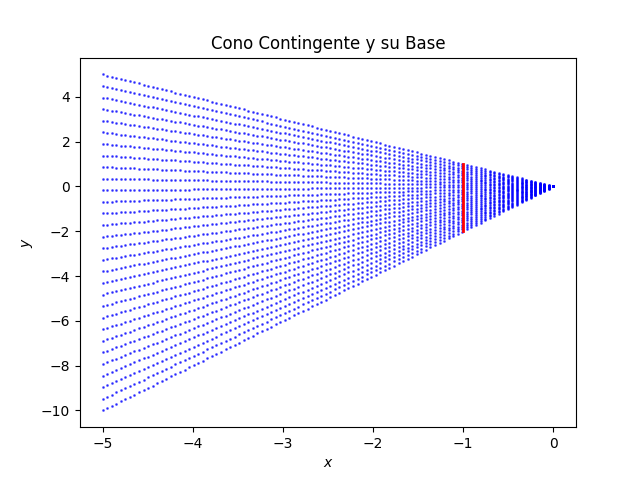
\includegraphics[scale=0.6]{pec3_ex2_TS.png}
\caption{
    Cono contingente y su base.
}
\label{ex2_plot_TS}
\end{figure}

	\section*{3}

\begin{definition}
    Sea $S$ un conjunto convexo no vacío de un espacio vectorial real y $f : S \rightarrow \R$.
    \begin{enumerate}[label=\textup{(\alph*)}]
        \item Pseudoconvexidad estricta.
            \textup{
                Supóngase que $f$ tiene derivada direccional en un punto $\bar{x} \in S$ en cada dirección $x - \bar{x}$,
                con $x \in S$.
                Se dice que f es estrictamente pseudoconvexo en $\bar{x}$ si
                \begin{equation*}
                    f'(\bar{x})(x - \bar{x}) \geq 0, \text{ para } x \in S, \; x \neq \bar{x} \Rightarrow f(x) > f(\bar{x}).
                \end{equation*}
            }
            
            \item Cuasi convexidad fuerte.
                \textup{
                    Se dice que $f$ es cuasi convexo fuerte en $S$ si para cada $x_1 , x_2 \in S$, con $x_1 \neq x_2$,
                    se tiene que
                    \begin{equation*}
                        f(\lambda x_1 + (1 - \lambda) x_2) < \max \{ f(x_1), f(x_2) \}, \text{ para cada } \lambda \in (0, 1).
                    \end{equation*}
                }
    \end{enumerate}
\end{definition}
Se pide probar el siguiente resultado:

\begin{theorem}
    Sea $S$ un conjunto convexo no vacío de un espacio vectorial normado.
    \begin{enumerate}[label=\textup{(\alph*)}]
        \item 
            \textup{
                Considérese el problema
                \begin{equation*}
                    \min_{x \in S} f(x),
                \end{equation*}
                con $f : S \rightarrow \R$.
                Supóngase que $f$ es cuasi convexo fuerte en $S$.
                Si $\hat{x}$ es un mínimo local del problema,
                entonces $\hat{x}$ es la única solución global del problema.
            }
    
        \item 
            \textup{
                Sea $f$ un funcional definido en un conjunto abierto que contiene a $S$.
                Si $f$ es diferenciable Fréchet en cada punto $\hat{x} \in S$ y estrictamente pseudoconvexo en cada punto $\hat{x} \in S$,
                entonces $f$ es cuasi convexo fuerte en $S$.
            }
    \end{enumerate}
\end{theorem}

\noindent\rule{10cm}{0.4pt}

\subsection*{(a)}

Este aparatado es muy similar al problema 2 de la entrega del bloque 1.

Sea $x_0 \in S$ un mínimo local de un funcional cuasi convexo fuerte $f$.
Entonces $\exists \varepsilon > 0$ tal que $f(x_0) \leq f(x)$ para todo $x \in S \cap B(x_0, \varepsilon)$.

Consideremos un punto $x \in S \setminus B(x_0, \varepsilon)$, tal que $f(x) \neq f(x_0)$.
Definimos $\lambda := \frac{\varepsilon}{\| x_0 - x \|} \in (0, 1)$,
obteniendo $x_\lambda := \lambda x + (1 - \lambda) x_0 \in S$,
\begin{equation*}
    \| x_\lambda - x_0 \| = \| \lambda x + (1 - \lambda) x_0 - x_0 \| = \lambda \| x - x_0 \| = \varepsilon,
\end{equation*}
es decir $x_\lambda \in B(x_0, \varepsilon)$.

Por tanto, como $x_0 \neq x_\lambda$, utilizando la cuasi convexidad fuerte de $f$,
\begin{equation*}
    f(x_0) \leq f(x_\lambda) = f(\lambda x + (1 - \lambda) x_0 - x_0) < \max \{ f(x), f(x_0) \},
\end{equation*}
lo que implica $f(x_0) < f(x)$, por tanto para todo $x \in S$ tenemos que $f(x_0) = f(x)$ o bien $f(x_0) < f(x)$,
asi que $x_0$ es un mínimo global.


\subsection*{(b)}

Para demostrar la segunda parte del teorema seguiremos la idea de la demostración del teorema 4.18 del texto base.

Dados $x, y \in S$ tales que $x \neq y$,
supongamos que existe $\hat{\lambda} \in (0, 1)$ tal que
\begin{equation*}
    f(\hat{\lambda} x + (1 - \hat{\lambda}) y) \geq \max \{ f(x), f(y) \}.
\end{equation*}
Como $f$ es diferenciable Fréchet,
por el teorema 3.15 del texto base $f$ es continua,
por tanto existe $\bar{\lambda} \in (0, 1)$ tal que
\begin{equation*}
    f(\bar{\lambda} x + (1 - \bar{\lambda}) y) \geq f(\lambda x + (1 - \lambda) y), \text{ para todo } \lambda \in (0, 1).
\end{equation*}

Usando el teorema 3.13 y el teorema 3.8 (a) del texto base tenemos que para $\bar{x} := \bar{\lambda} x + (1 - \bar{\lambda}) y$
\begin{equation*}
    f'(\bar{x})(x - \bar{x}) \leq 0,
\end{equation*}
y
\begin{equation*}
    f'(\bar{x})(y - \bar{x}) \leq 0.
\end{equation*}
Con
\begin{equation}\label{ex3_b_ineq}
\begin{aligned}
    x - \bar{x} & = x - \bar{\lambda} x - (1 - \bar{\lambda}) y = (1 - \bar{\lambda}) (x - y), \\
    y - \bar{x} & = y - \bar{\lambda} x - (1 - \bar{\lambda}) y = - \bar{\lambda} (x - y), \\
\end{aligned}
\end{equation}
usando la linearidad de $f'(\bar{x})$ obtenemos
\begin{equation*}
    0 \geq f'(\bar{x})(x - \bar{x}) = (1 - \bar{\lambda}) f'(\bar{x}) (x - y),
\end{equation*}
y
\begin{equation*}
    0 \geq f'(\bar{x})(y - \bar{x}) = - \bar{\lambda} f'(\bar{x}) (x - y).
\end{equation*}
Por tanto tenemos que $f'(\bar{x})(x - y) = 0$,
y usando la igualdad $(\ref{ex3_b_ineq})$ también tenemos $f'(\bar{x})(y - \bar{x}) = 0$.

Como hemos asumido que $f$ es estrictamente pseudoconvexo en cada punto $x \in S$,
$f$ es estrictamente pseudoconvexo en $\bar{x}$ y por tanto
\begin{equation*}
    f(y) - f(\bar{x}) > 0.
\end{equation*}

Pero esta desigualad contradice la siguiente desigualad
\begin{equation*}
\begin{aligned}
    f(y) - f(\bar{x})
        & = f(y) - f(\bar{\lambda} x + (1 - \bar{\lambda}) y) \\
        & \leq f(y) - f(\hat{\lambda} x + (1 - \hat{\lambda}) y) \\
        & \leq f(y) - \max \{ f(x), f(y) \} \\
        & \leq 0. \\
\end{aligned}
\end{equation*}

Por tanto para todo $\lambda \in (0,1)$
\begin{equation*}
    f(\lambda x + (1 - \lambda) y) < \max \{ f(x), f(y) \},
\end{equation*}
y consecuentemente $f$ es cuasi convexo fuerte.

\end{document}